\documentclass{article}
\usepackage{url}
\usepackage[utf8]{inputenc}
\usepackage{graphicx}
\usepackage{collcell}
\usepackage{listings}
\usepackage{amsmath}
\usepackage[margin = 0.5in]{geometry}
\usepackage{xcolor}

% Defines the colors that are used
\definecolor{comment_color}{rgb}{0,0.6,0}
\definecolor{number_color}{rgb}{0.5,0.5,0.5}
\definecolor{string_color}{rgb}{0.58,0,0.82}
\definecolor{backcolour}{rgb}{0.95,0.95,0.95}
\definecolor{nvidia_green}{HTML}{76b900}

% This is here in case we want to include code in the future
\lstdefinestyle{mystyle}{
    backgroundcolor=\color{backcolour},   
    commentstyle=\color{comment_color},
    keywordstyle=\color{magenta},
    numberstyle=\tiny\color{number_color},
    stringstyle=\color{string_color},
    basicstyle=\ttfamily\footnotesize,
    breakatwhitespace=false,         
    breaklines=true,                 
    captionpos=b,                    
    keepspaces=true,                 
    numbers=left,                    
    numbersep=5pt,                  
    showspaces=false,                
    showstringspaces=false,
    showtabs=false,                  
    tabsize=2,
    frame=tb
}

\lstset{style=mystyle}
\graphicspath{./imgs}
\title{Musically Composed Visuals-Design}
\author{Fourier2 Team}
\date{Spring 2023}

\begin{document}

\maketitle

\section{Team}
Justin Choi, Ryan Gaffney, Ian Lips, Matt Dim

\section{Goal}
Musically-Composed-Visuals Parallelizing audio transformation into different classifications regarding image generation and using graphics to display our results (in the form of fractals or other image processing). There are already ways of breaking music into components through fourier. These components would split songs into components such as basslines, vocals, accompaniment, etc.
\begin{figure}[!hbt]
    \centering
    \begin{tabular}{lccccc}
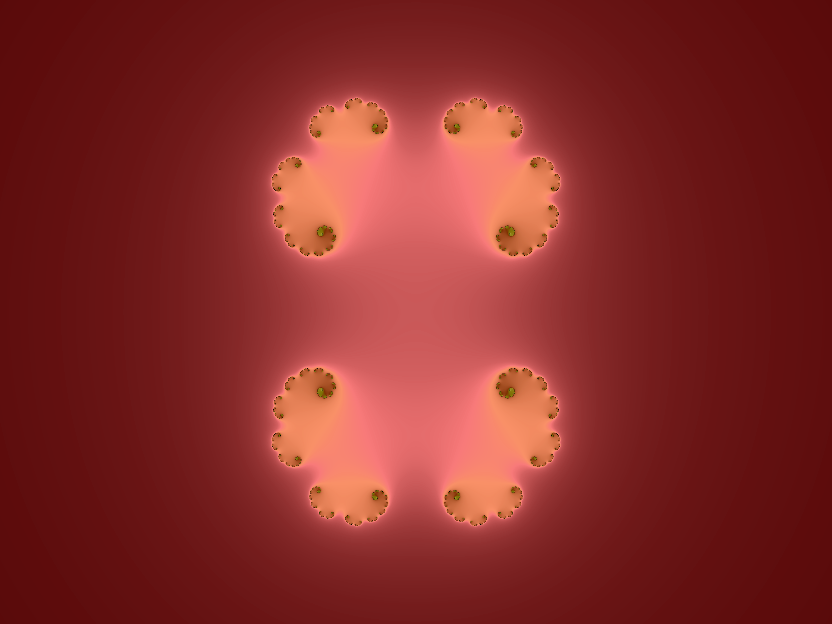
\includegraphics[scale = 0.15]{/imgs/image1.png}&

\includegraphics[scale = 0.15]{/imgs/image2.png}&
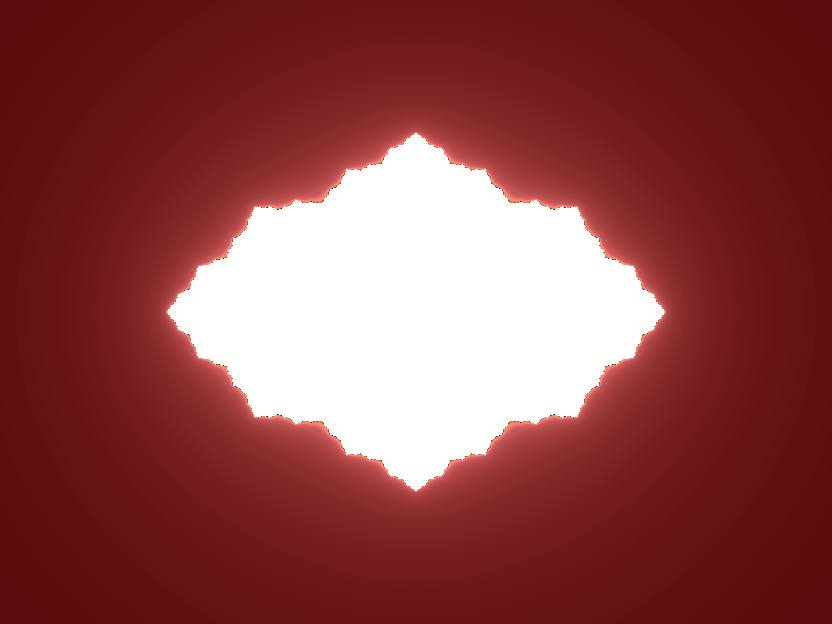
\includegraphics[scale = 0.15]{/imgs/image3.png}&

\end{tabular}
\caption{Polynomial Julia Set images}

\end{figure}

\section{Relevance}
OpenGL, a GPU library implementation talked about in the GPU part of the course, which will be used to animate our signal processed data to the screen. We will also be using both OpenMP and Pthreads for process speedup splitting up relevant tasks and data. This will be 

\section{Methods}
	We plan to use both OpenMP, Pthreads, and CUDA's managed memory to parallelize the processing of .mp3 and image generation. The data will be read from the src folder through native C I/O functions. We will then work on data and task parallelism in relevant sections of the signal processing functions. We expect that fourier transforms and audio compression will parallelize nicely because both of these functions are loops through data of the audio file. This means that we can have threads process different parts of a song at various points.
	Finally, we will use these processed signals and generate a mapping of audio to images. These images will be generated using OpenGL and we plan to use CUDA for parallelism. We will use the maximum kernels available on a machine for image generation of specific frames of a song. We hope to have an animation by the end that can be displayed per timestep. We will be performing testing during development in an incremental manner. 

\section{Possible Roadblocks}
The scale of the project is definitely a big roadblock to consider, as our plan is to generate a picture for virtually every point of a song, which could include up to thousands of images to process and generate. Through parallelism this will help with the massive amounts of gpu computation however we have never worked on a scale this large and may need to pivot to a smaller style of deliverable. For example instead of creating thousands of images for each point of a song, we can instead use the entirety of a song and its elements/components for one or a set of images. 


\section{Draft Deliverable}
For our draft, our submission will consist of an instance of a song that will be broken down into its components with all those components being parallelized and displayed into a single image. 

Significant progress would consist of the serial implementation being finished where we can display an image from a section of a song (or from any information from the song).
Excellent progress would be the implementation of threading and basic analysis on speedup with thorough testing. We would also include a serial version while getting openGL and cuda to communicate using the documentation from 
\textcolor{nvidia_green}{OpenGL Interoperability}.

\section{Final Deliverable}
Alongside our code and report, we will also be submitting an audio file and the images processed by that audio file. The audio file will be sent in its base form (most likely an MP3) and if we have time we can compare the different kinds of images created depending on the current parameters. We may even be able to show the images through an animated style by having each individual part of a song its own image.

\begin{thebibliography}{9}
\bibitem{OpenGl Interoperability}
N. Corporation, “OpenGL interoperability,” \emph{NVIDIA Documentation Hub}, 2023. [Online]. 
Available: \url{https://docs.nvidia.com/cuda/cuda-runtime-api/group__CUDART__OPENGL.html}. [Accessed: 03-Mar-2023]. 

\bibitem{K.Kolsha}
 K. Kolsha, “Kolsha/STM32-audio-visualizer: Audio visualizer based on stm32 and Extension Board.,” GitHub, 2018. [Online]. 
 Available: \url{https://github.com/Kolsha/STM32-AUDIO-VISUALIZER}. [Accessed: 03-Mar-2023]. 

\bibitem{C.Williams}
C. Williams, “Online fractal generator,” UsefulJS, 2014. [Online]. 
Available: \url{http://usefuljs.net/fractals/}. [Accessed: 03-Mar-2023]. 

\bibitem{ASENAULUG}
C. Zelga, A. Ulug, and J. Gilbert, “ASENAULUG/music-visualizer: A music visualizer which displays the real time fast Fourier transform (FFT) of music on an RGB led matrix,” GitHub, 2019. [Online]. 
Available: \url{https://github.com/asenaulug/music-visualizer}. [Accessed: 03-Mar-2023]. 


\end{thebibliography}

\end{document}